\documentclass[]{article}

\usepackage{caption}
\usepackage{graphicx, subfig}
\usepackage{listings}
\usepackage[namelimits]{amsmath} 
\usepackage{fontspec}
\usepackage{amsmath}
\usepackage{amssymb}                      
\usepackage{mathrsfs}  
\usepackage{amsfonts}   
\setmainfont[Mapping=tex-text]{KaiTi}
\usepackage{fullpage}
\usepackage{amsthm}
\usepackage{fancyhdr}
\usepackage{algorithm}
\usepackage{algorithmic}
\usepackage{bm}
\usepackage{ctex}
\usepackage{txfonts}

\usepackage[usenames,dvipsnames]{xcolor}

%opening
\title{统计机器学习 课后作业4}
\author{陈劭涵 17300180049}



\newcommand{\tm}{\fontspec{Times New Roman}}


\begin{document}
	
\maketitle


\section{问题1}
\begin{flushleft}
解:
\end{flushleft}
我们知道:\\\\
$p(x_i;\beta)=P(Y=1|X=x_i)=\frac{exp(x_i^T\beta)}{1+exp(x_i^T\beta)}$\\\\
所以有:\\\\
$\iota(\beta)=\sum_{i=1}^{N}\{y_ilogp(x_i;\beta)+(1-y_i)log(1-p(x_i;\beta))\}=\sum_{i}\{y_ilog\frac{exp(x_i^T\beta)}{1+exp(x_i^T\beta)}+(1-y_i)log(1-\frac{exp(x_i^T\beta)}{1+exp(x_i^T\beta)})\}$\\\\
$=\sum_{i}\{y_ix_i^T\beta-y_ilog(1+exp(x_i^T\beta))+(1-y_i)log(\frac{1}{1+exp(x_i^T\beta)})\}$\\\\
$=\sum_{i}\{y_ix_i^T\beta-y_ilog(1+exp(x_i^T\beta))+(y_i-1)(log(1+exp(x_i^T\beta))\}$\\\\
$=\sum_{i}\{y_ix_i\beta-log(1+exp(x_i^T\beta))\}$\\\\
那么我们就求出了蓝色部分
\section{问题2}
\begin{flushleft}
	解:
\end{flushleft}
我们先求二阶导数表达式:\\\\
课上已经求完了一阶导数的表达式:\\\\
$\frac{\partial l(\beta)}{\partial\beta}=\sum_{i}(y_ix_i-\frac{exp(x_i^T\beta)x_i}{1+exp(x_i^T\beta)})$\\\\
$\therefore \frac{\partial^2l(\beta)}{\partial\beta\partial\beta^T}=\sum_{i}\frac{\partial(\frac{x_i}{1+exp(x_i^T\beta)})}{\partial\beta^T}=\sum_i\frac{-exp(x_i^T\beta)x_ix_i^T}{(1+exp(x_i^T\beta))^2}$\\\\
把$p(x_i;\beta)=\frac{exp(x_i^T\beta)}{1+exp(x_i^T\beta)}$带到等式里\\\\
 $\frac{\partial^2l(\beta)}{\partial\beta\partial\beta^T}=-\sum_ix_ix_i^Tp(x_i;\beta)(1-p(x_i;\beta))$\\\\
The R codes:
\begin{lstlisting}[language=R]
# Problem 2 

# N-R algorithm for R=200 rounds
NR = function(N){
	beta = c(0.5, 1.2, -1)
	R = 200
	result = matrix(0,0,3)
	for (i in 1:R){
		X1 = rnorm(N)
		X2 = rnorm(N)
		X = cbind(1, X1, X2)  
		Y = exp(X%*%beta)/(1+exp(X%*%beta))
		for (j in 1: length(Y)){
			judge=runif(1,min=0,max=1)
			if (judge>Y[j]){
				Y[j]=0
			}
			if (judge<=Y[j]){
				Y[j]=1
			}
		}
		beta_old = c(-1, -1, -1) 
		beta_new = c(0.5, 0.5, 0.5)
		while(max(abs(beta_old-beta_new))>1e-5)
		{
			P = as.numeric(exp(X %*% beta_new)/(1+exp(X %*% beta_new)))  
			W = diag(P*(1-P))
			partial1 = t(X)%*%(Y-P)
			partial2 = t(X)%*%W%*%X
			beta_old = beta_new
			beta_new = beta_old+solve(partial2)%*%partial1
		}
		result=rbind(result,t(beta_new)) 
	}
	return(result)  
}

# calculate result for N=200,500,800,1000
NL=c(200,500,800,1000)
result1 = NR(NL[1]) 
result2 = NR(NL[2]) 
result3 = NR(NL[3]) 
result4 = NR(NL[4])

# do boxplot (recall that beta=c(0.5,1.2,-1))
boxplot(result1[,1]-0.5, result2[,1]-0.5, result3[,1]-0.5, result4[,1]-0.5, 
col="coral1", border="dimgray",
main="各轮次计算的beta_0与实际值差值的分布箱线图", ylab="hat(beta_0)-beta_0", 
names=c('N=200','N=500','N=800','N=1000'))

boxplot(result1[,2]-1.2, result2[,2]-1.2, result3[,2]-1.2, result4[,2]-1.2, 
col="dodgerblue", border="dimgray",
main="各轮次计算的beta_1与实际值差值的分布箱线图", ylab="hat(beta_1)-beta_1", 
names=c('N=200','N=500','N=800','N=1000'))

boxplot(result1[,3]+1, result2[,3]+1, result3[,3]+1, result4[,3]+1, 
col="mediumspringgreen",border="dimgray",
main="各轮次计算的beta_2与实际值差值的分布箱线图", ylab="hat(beta_2)-beta_2", 
names=c('N=200','N=500','N=800','N=1000'))

\end{lstlisting}
The results are:\\\\
	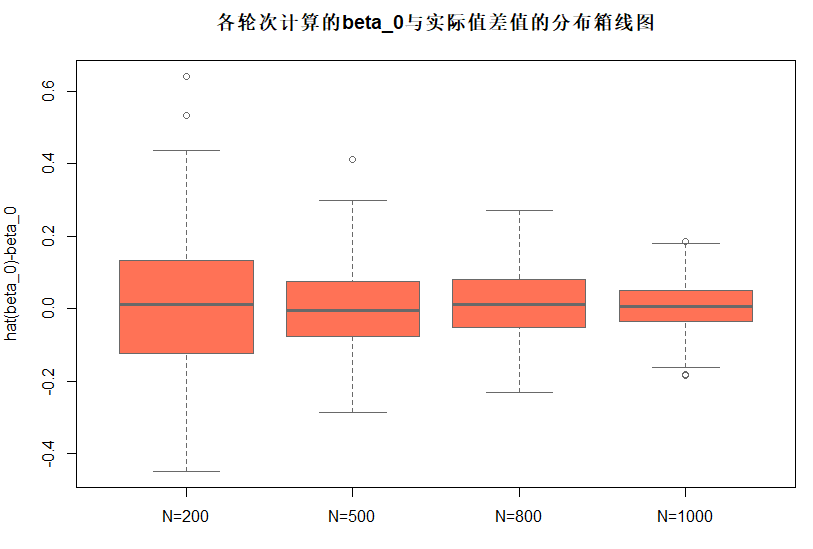
\includegraphics[width=.8\textwidth]{D:/大数据学院文件资料/2020秋课程/机器学习/homework/hw4/2.1.png}\\\\
	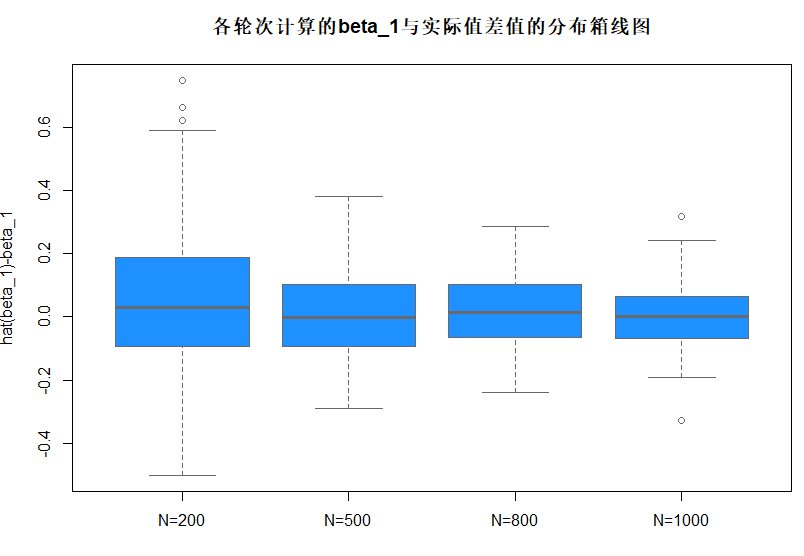
\includegraphics[width=.8\textwidth]{D:/大数据学院文件资料/2020秋课程/机器学习/homework/hw4/2.2.png}\\\\
	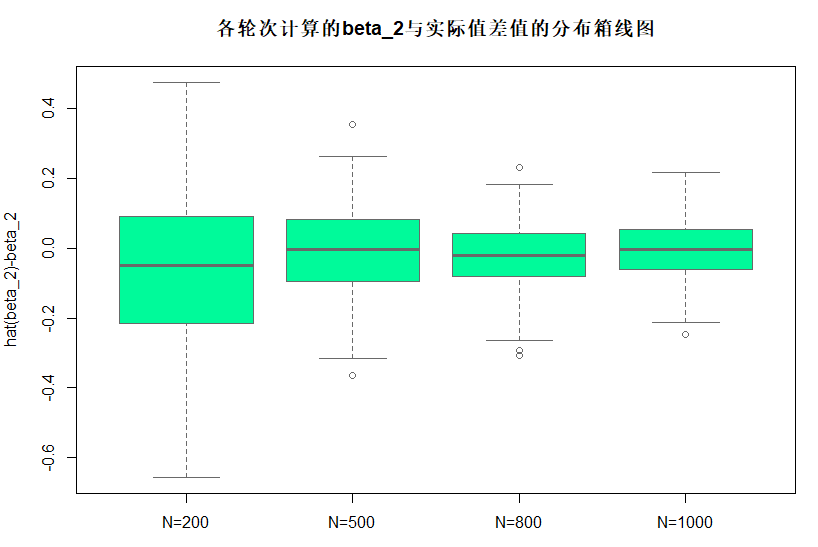
\includegraphics[width=.8\textwidth]{D:/大数据学院文件资料/2020秋课程/机器学习/homework/hw4/2.3.png}\\\\
从箱线图中我们可以看到$\hat{\beta}$通过NR算法,很好地往$\beta$收敛了,在200轮 模拟中得到的$\hat{\beta}$大部分都比较靠近$\beta$\\\\
此外随着N的增大,$\hat{\beta}$ 的分布更为集中和收缩,分布范围缩小了很多\\\\ 
\section{问题3}
\begin{flushleft}
	解:
\end{flushleft}
从ROC曲线的定义我们可以知道:\\\\
ROC曲线上方的面积等同于$m^{-}$个底为$\frac{1}{m^{-}}$,高为$\frac{1}{m^{+}}\times$剩余正例数的长方形的面积之和\\\\
$\therefore$ S(area above ROC)=$\sum_{x^+\in D^+}\sum_{x^-\in D^-}(\frac{1}{m^-}\times\frac{1}{m^+}\times I(f(x^+)<f(x^-)))$\\
=$\frac{1}{m^+m^-}\sum_{x^+\in D^+}\sum_{x^-\in D^-}(I(f(x^+)<f(x^-)))$=$l_{rank}$\\\\
$\therefore$ S(area under ROC)=AUC=1-S(area above ROC)=1-$l_{rank}$\\\\
\section{问题4}
\begin{flushleft}
	解:
\end{flushleft}
原始状态下,在训练集中有48393个观测样本,在测试集中有47900个测试样本\\\\
根据"expense", "tightness", "degree"变量的定义,它们都是大于0的正值\\\\
但是根据初步观察,发现数据集中有一些观测样本的这些变量值是小于0的负值,说明这些样本存在问题,但数量不是特别多。为了避免这些观测对后续分析的干扰,我们把他们筛除\\\\
筛除后,训练集中剩余48285个观测样本,测试集中剩余47771个观测样本\\\\
Problem(1) 读入数据:
\begin{lstlisting}[language=R]
# (1) read data
train=read.csv("D:/大数据学院文件资料/2020秋课程/机器学习/sampledata.csv")
\end{lstlisting}
Results:\\\\
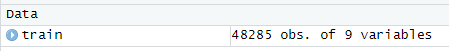
\includegraphics[width=.6\textwidth]{D:/大数据学院文件资料/2020秋课程/机器学习/homework/hw4/4.1.png}\\\\
Problem(2) 作箱线图:\\\\
为作图简洁,箱线图中的变量用英文表示;(备注:churn=1表示流失,churn=2表示不流失)
\begin{lstlisting}[language=R]
# (2) box plot
boxplot(log(tenure)~churn,data=train,col=c("dodgerblue","coral2"),
border=c("dimgray","dimgrey"),
main='log(tenure)~churn箱线图',names=c("churn=0","churn=1"),
xlab="churn or not",ylab="log(tenure)",plot=T)

boxplot(expense~churn,data=train,col=c("dodgerblue","coral2"),
border=c("dimgray","dimgrey"),
main='expense~churn箱线图',names=c("churn=0","churn=1"),
xlab="churn or not",ylab="expense",plot=T)

boxplot(log(degree)~churn,data=train,col=c("dodgerblue","coral2"),
border=c("dimgray","dimgrey"),
main='log(degree)~churn箱线图',names=c("churn=0","churn=1"),
xlab="churn or not",ylab="log(degree)",plot=T)

boxplot(log(tightness)~churn,data=train,col=c("dodgerblue","coral2"),
border=c("dimgray","dimgrey"),
main='log(tightness)~churn箱线图',names=c("churn=0","churn=1"),
xlab="churn or not",ylab="log(tightness)",plot=T)

boxplot(entropy~churn,data=train,col=c("dodgerblue","coral2"),
border=c("dimgray","dimgrey"),
main='entropy~churn箱线图',names=c("churn=0","churn=1"),
xlab="churn or not",ylab="entropy",plot=T)

boxplot(chgdegree~churn,data=train,col=c("dodgerblue","coral2"),
border=c("dimgray","dimgrey"),
main='chgdegree~churn箱线图',names=c("churn=0","churn=1"),
xlab="churn or not",ylab="chgdegree",plot=T)

boxplot(chgexpense~churn,data=train,col=c("dodgerblue","coral2"),
border=c("dimgray","dimgrey"),
main='chgexpense~churn箱线图',names=c("churn=0","churn=1"),
xlab="churn or not",ylab="chgexpense",plot=T)
\end{lstlisting}
Results are:\\\\
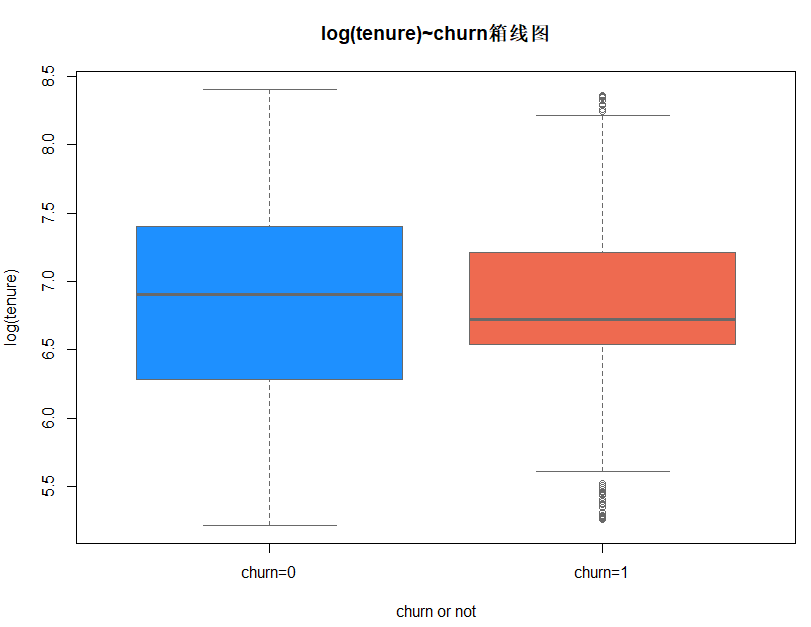
\includegraphics[width=.5\textwidth]{D:/大数据学院文件资料/2020秋课程/机器学习/homework/hw4/4.2.1.png}
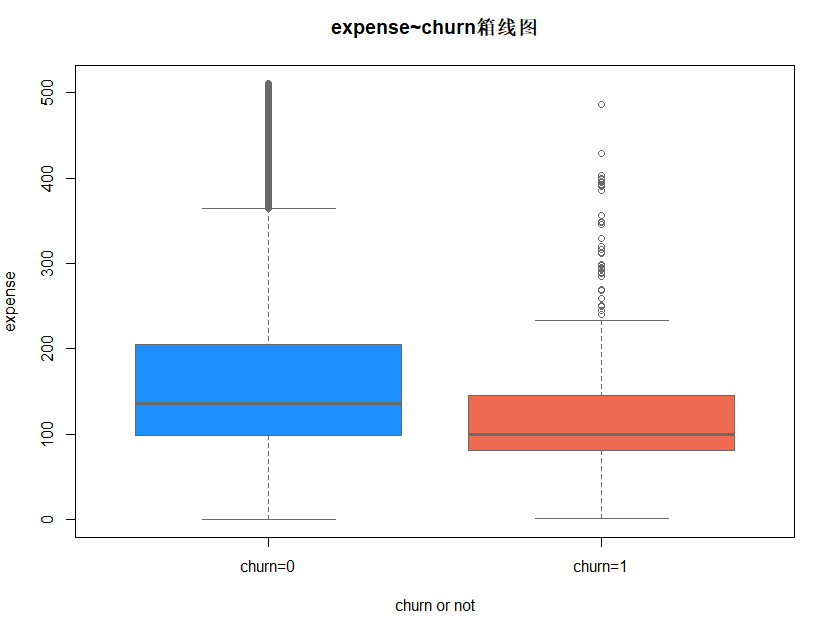
\includegraphics[width=.5\textwidth]{D:/大数据学院文件资料/2020秋课程/机器学习/homework/hw4/4.2.2.png}\\\\
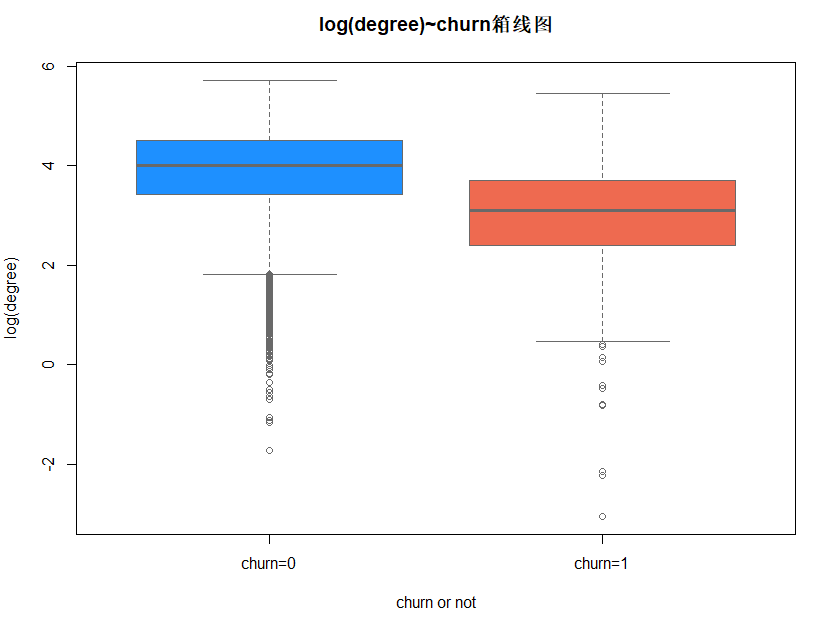
\includegraphics[width=.5\textwidth]{D:/大数据学院文件资料/2020秋课程/机器学习/homework/hw4/4.2.3.png}
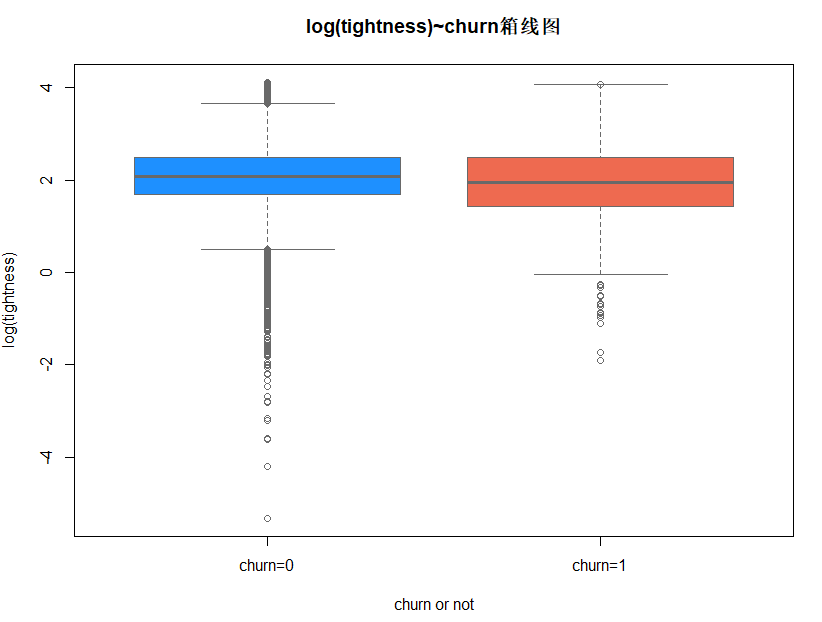
\includegraphics[width=.5\textwidth]{D:/大数据学院文件资料/2020秋课程/机器学习/homework/hw4/4.2.4.png}\\\\
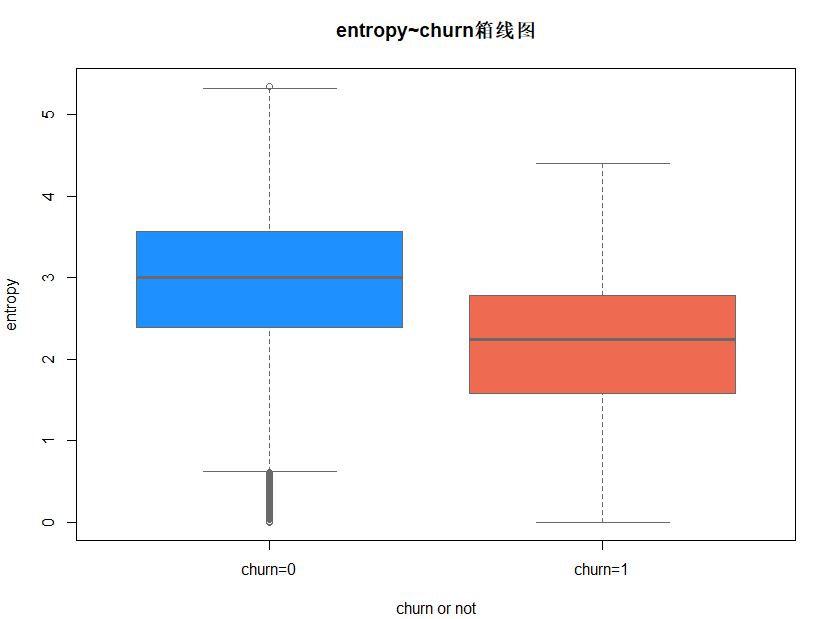
\includegraphics[width=.5\textwidth]{D:/大数据学院文件资料/2020秋课程/机器学习/homework/hw4/4.2.5.png}
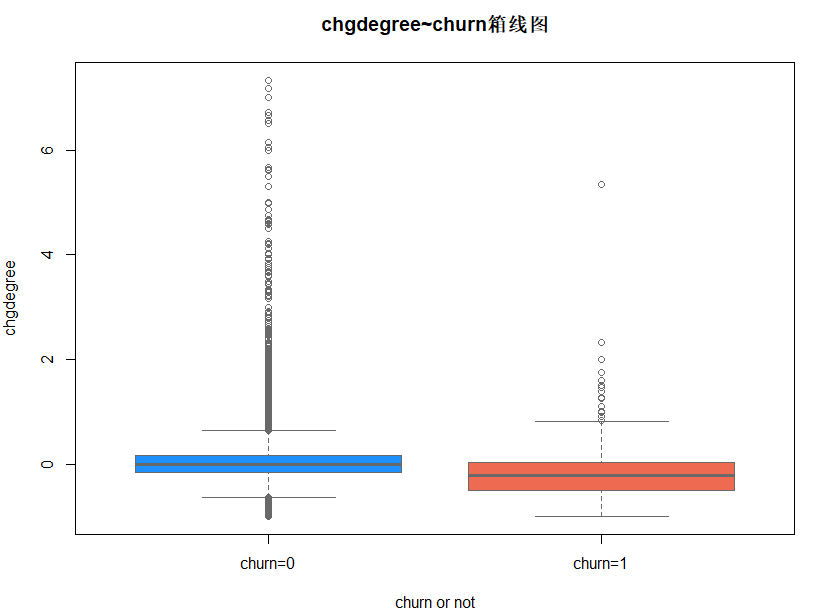
\includegraphics[width=.5\textwidth]{D:/大数据学院文件资料/2020秋课程/机器学习/homework/hw4/4.2.6.png}\\\\
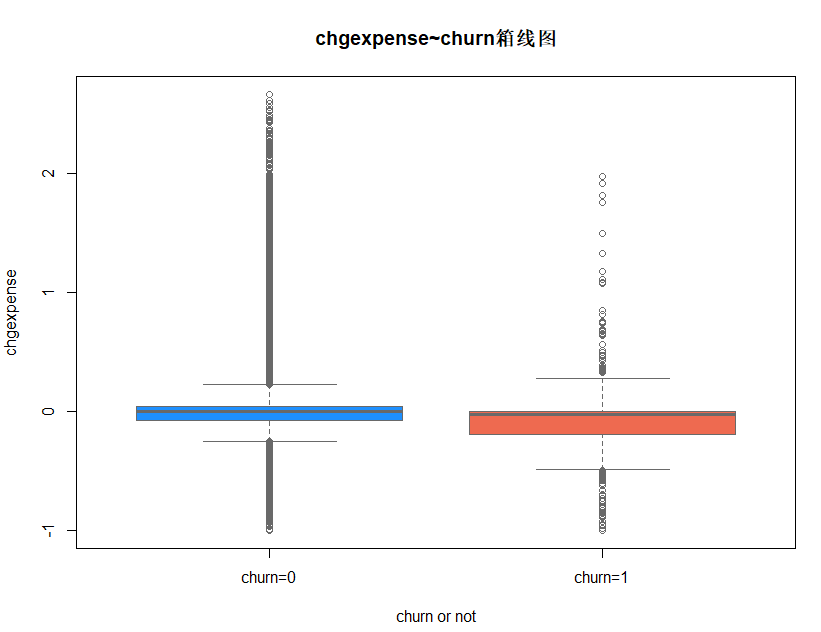
\includegraphics[width=.5\textwidth]{D:/大数据学院文件资料/2020秋课程/机器学习/homework/hw4/4.2.7.png}\\\\
从箱线图churn=1和churn=0的分布中我们可以看到:\\
1、在网时长相对较短的客户,更可能流失\\
2、当月话费较少的客户,更可能流失\\
3、和客户通话的总人数越少的客户,越可能流失\\
4、联系强度越少的客户流失的可能性相对较大,但不明显\\
5、个体信息熵越低的客户流失的可能性越大\\
6、个体度变化越低的客户,越可能流失\\
7、话费变化越低的客户,越可能流失\\\\
Problem(3) 标准化与逻辑回归:
\begin{lstlisting}[language=R]
# (3)
train[2:8]=scale(train[2:8])
reg_log=glm(churn~tenure+expense+degree+tightness+entropy+chgexpense+chgdegree,
data=train,family=binomial(link="logit")
)
summary(reg_log)
\end{lstlisting}
逻辑回归的参数结果是:
\begin{lstlisting}[language=R]
Call:
glm(formula = churn ~ tenure + expense + degree + tightness + 
entropy + chgexpense + chgdegree, family = binomial(link = "logit"), 
data = train)

Deviance Residuals: 
Min       1Q   Median       3Q      Max  
-0.8909  -0.1748  -0.1198  -0.0748   4.2072  

Coefficients:
Estimate Std. Error z value Pr(>|z|)    
(Intercept) -5.05338    0.07212 -70.067  < 2e-16 ***
tenure      -0.24767    0.06070  -4.080 4.50e-05 ***
expense     -0.29229    0.05904  -4.951 7.39e-07 ***
degree      -0.73751    0.13172  -5.599 2.15e-08 ***
tightness   -0.22660    0.04254  -5.327 9.99e-08 ***
entropy     -0.35176    0.07208  -4.880 1.06e-06 ***
chgexpense  -0.16071    0.04893  -3.284  0.00102 ** 
chgdegree   -0.38279    0.05208  -7.349 1.99e-13 ***
---
Signif. codes:  0 ‘***’ 0.001 ‘**’ 0.01 ‘*’ 0.05 ‘.’ 0.1 ‘ ’ 1

(Dispersion parameter for binomial family taken to be 1)

Null deviance: 6475.5  on 48284  degrees of freedom
Residual deviance: 5757.6  on 48277  degrees of freedom
AIC: 5773.6

Number of Fisher Scoring iterations: 8
\end{lstlisting}
解读:\\\\
1、从结果上看,对因变量“是否流失”而言,所有的这些变量在逻辑回归模型中都有较高的显著性水平(0.01和0.001)\\
2、模型截距项参数为-5.0534;自变量的系数估计分别为:\\
在网时长的系数-0.2476\\
当月话费系数-0.2923\\
个体的度系数-0.7375\\
联系强度系数-0.2266\\
个体信息熵系数-0.3518\\
个体度的变化系数-0.1607\\
花费的变化系数-0.3828\\
可以看到这些系数均小于0,这与箱线图中展示出的分布差异与初步结论也比较一致\\\\
Problem(4) 逻辑回归预测
\begin{lstlisting}[language=R]
# (4)
train_pred=predict.glm(reg_log,newdata=train,type="response")
head(train_pred)
test=read.csv("D:/大数据学院文件资料/2020秋课程/机器学习/preddata.csv")
test[2:8]=scale(test[2:8])
test_pred=predict.glm(reg_log,newdata=test,type="response")
head(test_pred)
\end{lstlisting}
预测结果(开头的一部分):
\begin{lstlisting}[language=R]
> head(train_pred)
1           2           3           4           5           6 
0.004999719 0.010796015 0.003467837 0.008023648 0.002977289 0.001469916 
\end{lstlisting}
\begin{lstlisting}[language=R]
> head(test_pred)
1            2            3            4            5            6 
0.0332009167 0.0062862747 0.0085627283 0.0006695617 0.0073670728 0.0037128759 
\end{lstlisting}
train\_pred和test\_pred就是预测流失概率值的向量\\\\
Problem(5) 绘制ROC曲线与AUC计算
R codes:
\begin{lstlisting}[language=R]
# (5)
library("pROC")

roc(train$churn,train_pred,plot=TRUE,main="训练集ROC曲线",xlab = "FPR", ylab = "TPR",
print.thres=TRUE,print.auc=TRUE,legacy.axes=TRUE,grid=c(0.2,0.2),
grid.col="dimgray",auc.polygon=TRUE,max.auc.polygon=TRUE,
auc.polygon.col="darkslategray1",max.auc.polygon.col="deepskyblue")

roc(test$churn,test_pred,plot=TRUE,main="测试集ROC曲线",xlab = "FPR", ylab = "TPR",
print.thres=TRUE,print.auc=TRUE,legacy.axes=TRUE,grid=c(0.2,0.2),
grid.col="dimgray",auc.polygon=TRUE,max.auc.polygon=TRUE,
auc.polygon.col="darkslategray1",max.auc.polygon.col="deepskyblue")
\end{lstlisting}
ROC曲线绘制的结果报告:
\begin{lstlisting}[language=R]
Call:
roc.default(response = train$churn, predictor = train_pred, plot = TRUE,     main = "训练集ROC曲线", xlab = "FPR", ylab = "TPR", print.thres = TRUE,     print.auc = TRUE, legacy.axes = TRUE, grid = c(0.2, 0.2),     grid.col = "dimgray", auc.polygon = TRUE, max.auc.polygon = TRUE,     auc.polygon.col = "darkslategray1", max.auc.polygon.col = "deepskyblue")

Data: train_pred in 47683 controls (train$churn 0) < 602 cases (train$churn 1).
Area under the curve: 0.7728

Call:
roc.default(response = test$churn, predictor = test_pred, plot = TRUE,     main = "测试集ROC曲线", xlab = "FPR", ylab = "TPR", print.thres = TRUE,     print.auc = TRUE, legacy.axes = TRUE, grid = c(0.2, 0.2),     grid.col = "dimgray", auc.polygon = TRUE, max.auc.polygon = TRUE,     auc.polygon.col = "darkslategray1", max.auc.polygon.col = "deepskyblue")

Data: test_pred in 47111 controls (test$churn 0) < 660 cases (test$churn 1).
Area under the curve: 0.7818
\end{lstlisting}
对应的训练集上和测试集上的ROC图:\\\\
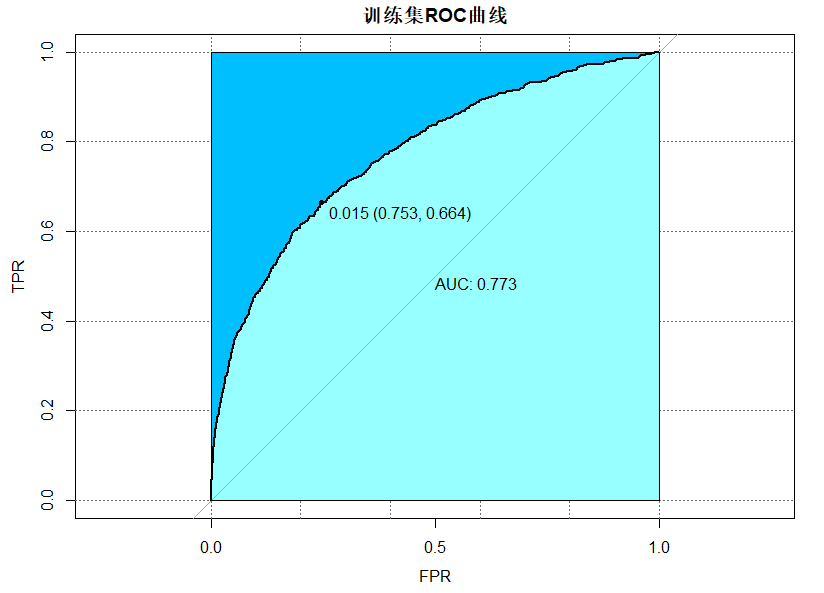
\includegraphics[width=.85\textwidth]{D:/大数据学院文件资料/2020秋课程/机器学习/homework/hw4/4.5.1.png}\\\\
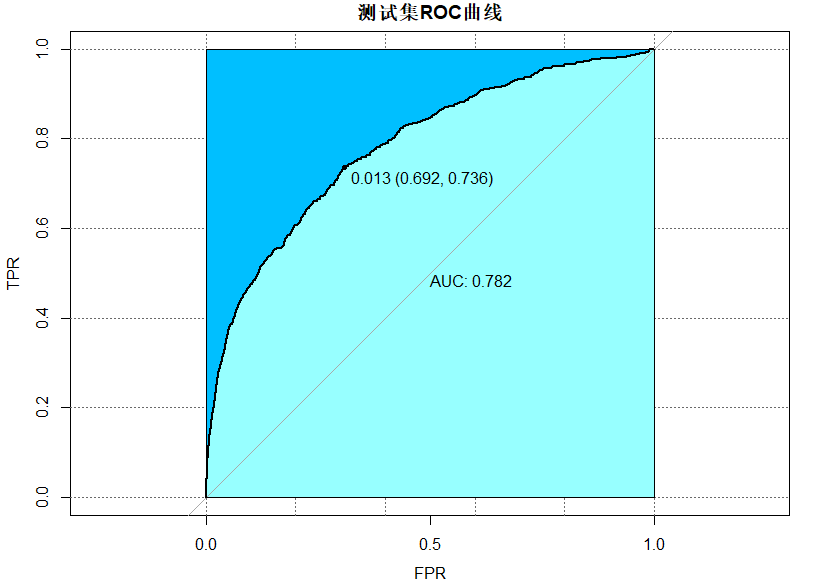
\includegraphics[width=.85\textwidth]{D:/大数据学院文件资料/2020秋课程/机器学习/homework/hw4/4.5.2.png}\\\\
计算AUC:
\begin{lstlisting}[language=R]
AUC_c = function(TP, FP){
	lrank = 0
	for (i in 1:length(TP))
	{
		lrank = lrank+1*sum(FP>TP[i]) + 0.5*sum(FP == TP[i])
	}
	lrank = 1 - lrank/ (length(TP) * length(FP))
	return(lrank)
}	
train_TP = train_pred[(train$churn==1)]
train_FP= train_pred[(train$churn==0)]
AUC_c(train_TP,train_FP)

test_TP = test_pred[(test$churn==1)]
test_FP= test_pred[(test$churn==0)]
AUC_c(test_TP,test_FP)
\end{lstlisting}
\begin{lstlisting}[language=R]
> AUC_c(train_TP,train_FP)
[1] 0.7728054
> AUC_c(test_TP,test_FP)
[1] 0.7818464
\end{lstlisting}
计算出的AUC与roc函数自动计算出的AUC吻合\\\\
根据ROC曲线和AUC值,我们看到模型在训练集上表现出了较好的预测效果(AUC=0.773)\\
此外模型在数据规模与训练集差不多的测试集上也一样表现出恶较好的预测效果(AUC=0.782),说明该模型的泛化能力还比较不错
\end{document}
